\chapter{Experiments} \label{chap:experiments}

In this section, we will be introducing the experiment we are conducting as well as showcasing different steps we are undertaking in order to conduct our experiment. Firstly, we will introduce the background leading to the experiment and the motivation behind this experiment. After that, we will list out the goals and expectations from the experiment as well as our hardware and software environment configuration. Then, we will setup the start conducting the experiment while simultaneously explaining and justifying each of the steps during the process.

After the experiment, we will first collect all the data that was produced from the experiment. We will than start analysing and categorising the collected data, process them and present them in the "Result" section. After that, we will provide our verdict of the experiment by delivering discussions on the experiment topic such as whether the result was largely within our expectation or perhaps the results differs from our initial assumption and prediction by a considerable margin.

Finally, we will finish off this section by listing the challenges we faced and the irregularities we found during our experiment, as well as possible future work that might be worth undertaking.

\bigskip
\bigskip

\textbf{{\Large Chapter 4.1 Background}}

\bigskip

In the above chapters, we have introduced the concept of WebAssembly, conducted detailed literature reviews on WASM and other related topics as well as conducted evaluation on the topics. Our experiment will be conducted in a controlled computer environment as well as in a real life scenario where the application will be deployed to the servers around the world for testing and benchmarking.

This way, we will be extra confident with the data we collected from the experiment and therefore, we will have a stronger argument when communicating our result to other researchers as well as making sure the result we got is as accurate as possible.

\bigskip
\bigskip

\textbf{{\Large Chapter 4.2 Motivation}}

\bigskip

Edge computing is getting popular day by day, according to Google searches, we are about 4 time more interested in edge computing than we were just 5 years ago [34]. Large network infrastructure and tech companies have also released edge computing frameworks and products, such as Google with Firebase Cloud Functions [35], Cloudflare with Cloudflare workers [36] and Vercel - The creator for Next.js [37], one of the most popular web frameworks, recently entered the edge computing market by introducing edge function for the framework [39].

However, with the current technology, hosting applications on the edge is just very inefficient. For example, according to Gadepalli et al. [39], the majority of the current implementation approach is either VM-Based or Container-Based.

For VM-Based implementation, each applications are hosted in virtual machines within a physical hardware. Each virtual machine consists of its own operating system, kernel resource management, library dependencies and language runtimes. All of these resources will then be used to run the application from the client. The physical hardware manages each of these virtual machines, for example, distributing memory and CPU usages and is known as a VM manager. This approach is used by a number of well-known PaaS (Platform as a service) providers. For example, AWS Lambda and Azure Functions [40] [41].

Container-Based implementation uses a more straight forward structure than VM-Based implementation. With Container-Based implementation, each applications will be hosted in containers as per name suggested. Each containers also contains its own library dependencies as well as language runtimes. However, unlike the virtual machine approach, containers have access directly to the hardware's memory and CPU as well as limited access to certain system APIs. With this method, applications are no longer hosted in virtual machines, therefore usually have a faster cold start latency than VM-Based approach. Popular services such as Google Cloud Function and Apache OpenWhisk uses this approach [42] [43].

After getting familiarised with the current technology, my natural research instinct kicked in, I kept asking myself if this is something that can be looked into and perhaps to be researched and experimented. From all the readings and literature reviews, it is easy to assume that WebAssembly simply has a better performance than the current technology including when running on the edge. However, we don't know the answer yet as this is only an assumption. Therefore, we are interested in comparing the performance between the two and we would like to conduct experiments in environments and scenarios described above.

\bigskip

\begin{figure}[hp]
\centering
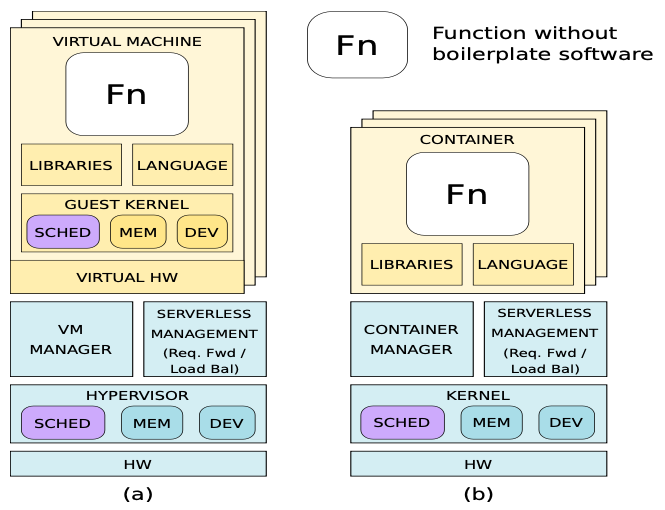
\includegraphics[scale=0.5]{sledge-design-a-b}
\caption{\footnotesize{Visualisation of the current edge computing system design layout, a: VM-Based implementation, b: Container-Based implementation}}
\captionsetup{aboveskip=0pt,font=it}
\label{fig:javascript_meme}
\end{figure}

\bigskip
\bigskip

\textbf{{\Large Chapter 4.3 Configuration and Further Understanding}}

\bigskip

Our experiment will focus on two kinds of microservice frameworks: VM/Container based frameworks and WebAssembly based frameworks. As stated above, we will conduct our research in two scenarios: experimental benchmark and real life testing. We will also run the benchmark tests both locally and on the edge servers.

Here are some of the WebAssembly frameworks we are interested in, we will conduct our experiment with one or multiple frameworks listed in the table below:

\bigskip

\begin{table}[h!]
\centering
\begin{tabular}{||c c c||} 
\hline
Name & Developer & Website \\ [0.5ex] 
\hline\hline
 & & \\
Sledge & George Washington University & https://github.com/gwsystems/sledge-serverless-framework \\ 
 & & \\
Spin & Fermyon & https://github.com/fermyon/spin \\
 & & \\
WasmEdge & Linux foundation & https://wasmedge.org/ \\
 & & \\
Krustlet & Deislabs & https://krustlet.dev/ \\
 & & \\
WAGI & Deislabs & https://github.com/deislabs/wagi \\
 & & \\
Wasmcloud & Wasmcloud team & https://wasmcloud.dev/ \\ [1ex] 
\hline
\end{tabular}
\caption{List of WebAssembly frameworks of interest}
\label{table:1}
\end{table}

\bigskip

A web framework, sometimes also referred as a web application framework, is a collection of functionalities and libraries that is engineered and designed with the intention of laying the groundwork and providing basic infrastructures and logic that is used in almost any software such as the ability to render graphical interface or to initialise communication to servers, which will be used to support the software that builds on top of it [44].

There are usually two categories of web frameworks: client-side framework and server-side framework. The former is usually used in order to construct dynamic web applications [45] while the latter is usually used to develop back-end API services. According to 2022 annual developer survey from stack overflow, some of the most popular client-side frameworks including React.js, Angular and Vue.js while some of the most popular server-side frameworks including Node.js, ASP.NET and Django (server-side Django REST framework) [46] [47] [48] [49] [50] [51] [52] [53].

It has been mentioned in multiple research articles that running full web applications using the current cloud solution may produce too much overhead, thus leads to inefficiency. For example, Gackstatter [54] recognise the limitation of today's "cloud-centric model" when it comes to deploying web applications at the edge. Specifically, the author stated that applying the current solution such as virtual machines and containers does not promise to be an effective solution due to limited resources available. Additionally, Gadepalli et al. not only pointed out the widely adoption of the virtual machine/container model, but also stated that server applications built using WASM functions that runs naively have the potential to expand the current use case of comprehensive applications running from the edge due to the reduction of the overhead which reduce the respond time down to within 10 milliseconds [39].

With the current model of implementation, docker or Kubernetes are usually used in the process in order to prepare an application for edge deployment. This would "wrap" the application into containers which will be further deployed onto self-managed serverless infrastructures or cloud services that provides edge services such as Amazon Web Service or Microsoft Azure to be distributed to edge devices across data centres around the world.

The topic and question of my research is to discover the performance gap and inconsistency between the current model of edge applications which includes application development and deployment with virtual machines, containers and traditional language runtimes, and the proposed WebAssembly solution which is to run functions as microservices directly from the native operating system using WebAssembly through a WASM runtime.

Currently at this stage, the true performance capability of WebAssembly has not yet been realised due to the relatively short time it has been around in comparison to JavaScript - which has almost 30 years of development. However, it is apparent to us that WebAssembly have a huge potential in terms of it's performance both when running in web browsers as well as running on operating systems naively through a runtime. We are able to back this up with the performance data of JavaScript over the years. In a presentation, Verschore presented a figure which stated that between 2001 and 2009, there was an 100-times improvement in JavaScript's performance as well as huge increases in the browser Octane score (web page loading speed) [55].

\begin{figure}[!ht]
\centering
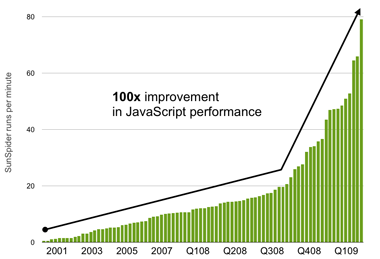
\includegraphics[scale=0.5]{js-perf}
\caption{\footnotesize{SunSpider benchmark score for the SpiderMonkey engine which is used in the Firefox browser}}
\captionsetup{aboveskip=0pt,font=it}
\label{fig:javascript_meme}
\end{figure}

\bigskip
\bigskip

On top of that, the JavaScript engine behind popular browsers such as Google Chrome [56] and Brave [57] - V8 [58], also had an incredible journey from when its first released to the public in 2008. The V8 development team undertook and released a set of benchmark scores comparing the performance of the Chrome browser from it's original beta to the versions in 2018. The results showed that in just 10 years, both its V8 Bench score [59] and Speedometer score [60] increased by 4 times and the engine had also became a lot more stable as well as added support for a lot more chip architectures such as ARM and ARM 64 [61] [62].

\bigskip

\begin{figure}[hp]
\centering
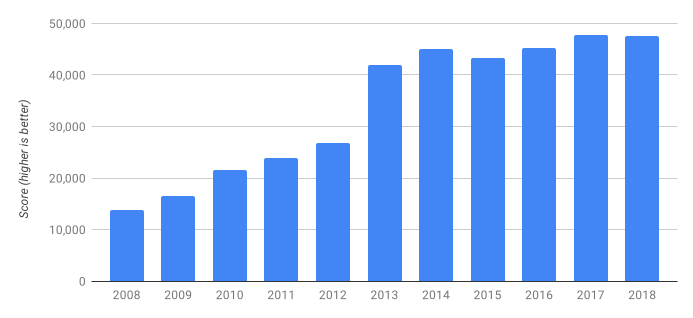
\includegraphics[scale=0.5]{chrome-v8-bench}
\caption{\footnotesize{Google Chrome's V8 Bench score between its original beta and the version in 2018}}
\captionsetup{aboveskip=0pt,font=it}
\label{fig:javascript_meme}
\end{figure}

\bigskip
\bigskip

\bigskip

\begin{figure}[hp]
\centering
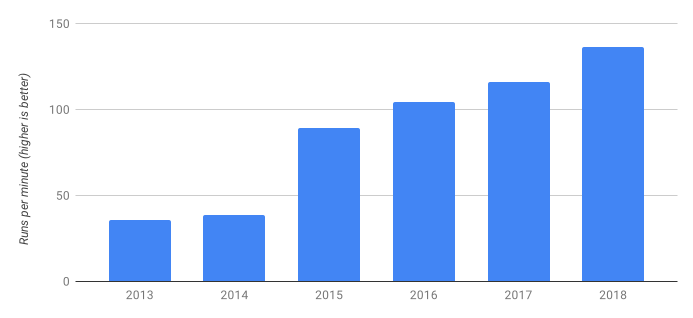
\includegraphics[scale=0.5]{chrome-speedometer-1}
\caption{\footnotesize{Google Chrome's Speedometer 1 score between its original beta and the version in 2018}}
\captionsetup{aboveskip=0pt,font=it}
\label{fig:javascript_meme}
\end{figure}

\bigskip
\bigskip

One of the recent example is 

\bigskip
\bigskip
\bigskip
\bigskip
\bigskip
\bigskip

Just like WebAssembly, developers started to use JavaScript outside of web browsers. Currently the most popular bring Node JS (https://nodejs.org/en/), followed by deno (https://deno.land/) with the newest release Bun js which "claims that it is able to perform 3 times faster than node js" (https://bun.sh/).

I would like this experiment to be the "Main" experiment. After setting up and conducting the experiment, we will then decide whether to conduct more experiments or this is significance enough. During the experiment, I will be writing up the report at the same time (especially during the setup process) to document as well as to record data.

The experiment will have be run under two scenarios: the first scenario is the benchmark test and the second scenario is a real life edge computing use case.

On the extra end, I will be using wrk (https://github.com/wg/wrk) which is a a HTTP benchmarking tool to measure more stats from each frameworks.

In terms of the framework setup, I will be using Python with FastAPI (https://fastapi.tiangolo.com/) for the traditional framework setup. With the WebAssembly frameworks, I will be using Sledge by GWU and Spin by Fermyon (I might throw in Wasmcloud if I have extra time).

I might need some help from Dr Thilakarathna when setting up for edge deployment, since I feel like I'm still really new in this area.

The first scenario (test) is a benchmark test, we will be using PolyBench/C (https://web.cse.ohio-state.edu\newline/pouchet.2/software/polybench/) and PolyBench/Python (https://github.com/UDC-GAC/polybench-python) and all code will be written in C and Python.

PolyBench was developed by Louis-Noël Pouchet from Colorado State University. It is consisted of 30 function tests that can run by itself without any external libraries:

- 2mm	2 Matrix Multiplications (D=A.B; E=C.D)\newline
- 3mm	3 Matrix Multiplications (E=A.B; F=C.D; G=E.F)\newline
- adi	Alternating Direction Implicit solver\newline
- atax	Matrix Transpose and Vector Multiplication\newline
- bicg	BiCG Sub Kernel of BiCGStab Linear Solver\newline
- cholesky	Cholesky Decomposition\newline
- correlation	Correlation Computation\newline
- covariance	Covariance Computation\newline
- doitgen	Multiresolution analysis kernel (MADNESS)\newline
- durbin	Toeplitz system solver\newline
- dynprog	Dynamic programming (2D)\newline
- fdtd-2d	2-D Finite Different Time Domain Kernel\newline
- fdtd-apml	FDTD using Anisotropic Perfectly Matched Layer\newline
- gauss-filter	Gaussian Filter\newline
- gemm	Matrix-multiply C=alpha.A.B+beta.C\newline
- gemver	Vector Multiplication and Matrix Addition\newline
- gesummv	Scalar, Vector and Matrix Multiplication\newline
- gramschmidt	Gram-Schmidt decomposition\newline
- jacobi-1D	1-D Jacobi stencil computation\newline
- jacobi-2D	2-D Jacobi stencil computation\newline
- lu	LU decomposition\newline
- ludcmp	LU decomposition\newline
- mvt	Matrix Vector Product and Transpose\newline
- reg-detect	2-D Image processing\newline
- seidel	2-D Seidel stencil computation\newline
- symm	Symmetric matrix-multiply\newline
- syr2k	Symmetric rank-2k operations\newline
- syrk	Symmetric rank-k operations\newline
- trisolv	Triangular solver\newline
- trmm	Triangular matrix-multiply\newline

All the tests are available in C and Python.

After that, I will then develop a real-life scenario application. I have yet to finalise the design of this application and I will be developing this application from this week.

I will collect as much data as possible and to present those data using a variety of graphs and charts.

Finally, I will run the performance stats test with wrk.

This is the proposal for the experiment. I believe including the time I will be spending writing the report and thesis, it would take me about two and a half weeks to finish.

After finalise the proposal, we will start the experiment immediately.

Thanks,\newline
Richard Lee